%----------------------------------------------------------------------------------------------------------------------------------
\subsection{Quantitative Analysis}\label{sec:qanalysis}
%----------------------------------------------------------------------------------------------------------------------------------

This section discusses the quantitative analysis that we propose as a result of applying the Systematic Mapping methodology.
Quantitative results are aggregated and presented in bubble charts that combined different facets. The combination of facets was done for answering the research questions proposed for guiding our study.

%Our analysis presents the frequencies of publications for
%the choosen facets. The charts show the aggregated view of the number of papers 
%considering the facets. This approach will help answer the three research
%questions more objectively.

 
%  . .  .  . .  .  . .  .  . .  .  . .  .  . .  .  . .  .  . .  .  . .  .  . .  .  . .  .  . .  .  . .  .  . .  .  . .  .  . .  .  . .  .  . .  .  . .  .  . .  .  . .  .  . .  .
\subsubsection{\textit{RQ1: Which are the SLA measures that have been mostly
applied  in the cloud?}}
%  . .  .  . .  .  . .  .  . .  .  . .  .  . .  .  . .  .  . .  .  . .  .  . .  .  . .  .  . .  .  . .  .  . .  .  . .  .  . .  .  . .  .  . .  .  . .  .  . .  .  . .  .  . .  .
\begin{figure}[h!]
\centering
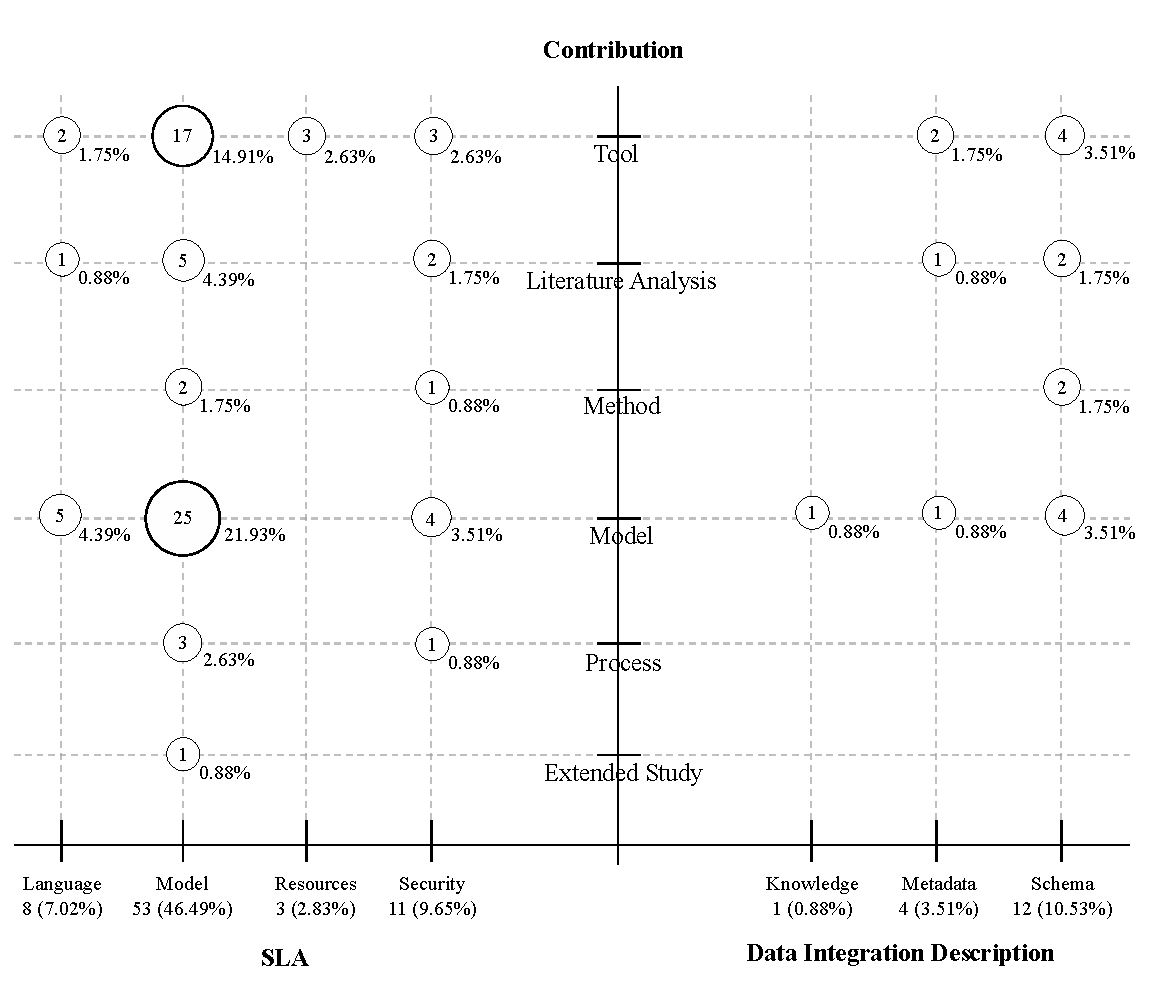
\includegraphics[scale=0.56]{figs/bubble-charts/Contribution-SLA-DIdescription.pdf} 
\caption{Contribution, SLA and Data Integration Description}\label{fig:facet1}
\end{figure}

The facets SLA expression, data integration description and contribution give elements for determining which SLA measures have been applied to the cloud   (Figure~\ref{fig:facet1}). The resulting bubble chart shows that most contributions propose SLA models and that  \textit{privacy}
and \textit{security} (11 appearances - 9.65\%) are the most popular measures considered by SLA models for the cloud. These measures concern the network, information, data protection and confidentiality in the cloud. Most contributions propose SLA models (53 appearances - 46.49\%)  but some languages (8 appearances - 7.02\%) have also emerged. {\em Data provenance} is also a measure that emerges but only in papers dealing with multi-cloud environments. Data integration is merely addressed by using schemata (12 appearances - 10.53\%)  and meta-data (4 appearances - 3.51\%) particularly through models (34 appearances - 29.82\%) and tools (25 appearances - 21.93\%). Still, some works propose literature studies (8 appearances - 7.02\%).
 
%The most used type of environment is \textit{cloud}, followed by \textit{data
%warehouse, multi-cloud} and \textit{federated database}. Looking to the figure
%you can alse note that models for SLA have been the focus in the papers (53 appearances - 46.49\%) followed by Security (11 appearances - 9.65\%), Language 
%(8 appearances - 7.02\%) and Resources (3 appearances - 22.83\%).
%Analyzing the figure is also possible to observe that Model (34 appearances - 29.82\%) and 
%Tool (25 appearances - 21.93\%) are the mainly type of contribution proposed in the papers 
%followed by Literature Analysis (8 appearances - 7.02\%), Process (4 appearances - 3.51\%), 
%Method (3 appearances - 2.63\%) and Extended Study (1 appearance - 0.88\%).

%Regarding the data integration description, Schema (12 appearances - 10.53\%) is
%the most applied dimension followed by Metadata (4 appearances - 3.51\%) and
%Knowledge (1 appearance - 0.88\%).

%The limitation of cloud applications, considering SLAs, is the difficulty in
%determining main reason for service interruptions due to the complex of
%the environment. Even so, there are few works that consider \textit{data
%protection} in such cases. One of the challenges of apply SLA in cloud
%environments is to find the specific need of the application, so as to attack
%the solution (\textit{security, privacy, confidentiality, data protection} or
%\textit{data provenace}) in a objectively way, by proposing SLA models, methods,
%or even new tools.

%  . .  .  . .  .  . .  .  . .  .  . .  .  . .  .  . .  .  . .  .  . .  .  . .  .  . .  .  . .  .  . .  .  . .  .  . .  .  . .  .  . .  .  . .  .  . .  .  . .  .  . .  .  . .  .
\subsubsection{\textit{RQ2: How have published papers on data integration evolved towards cloud topics?}}
%  . .  .  . .  .  . .  .  . .  .  . .  .  . .  .  . .  .  . .  .  . .  .  . .  .  . .  .  . .  .  . .  .  . .  .  . .  .  . .  .  . .  .  . .  .  . .  .  . .  .  . .  .  . .  .
\begin{figure}[h]
\centering
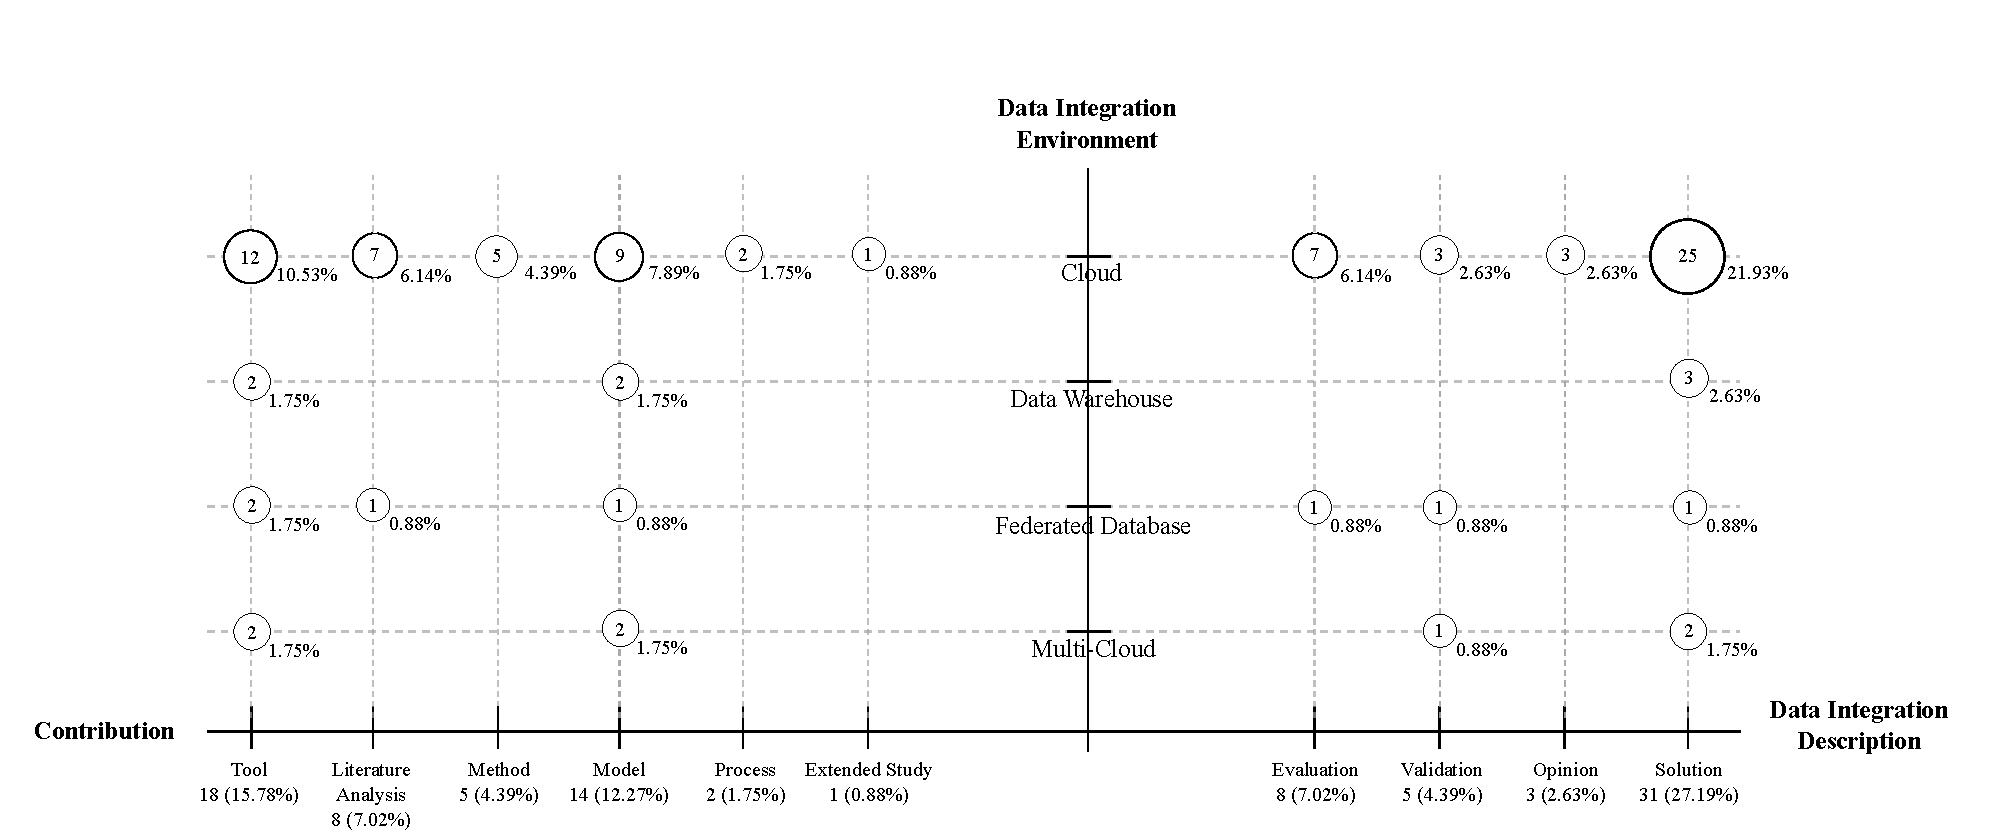
\includegraphics[scale=0.48]{figs/bubble-charts/DI-Environment-Contribution-Research.pdf}
\caption{facets Data Integration Environment, Contribution and Research}\label{fig:facet2}
\end{figure}

Combining the facets data integration environment, contribution
and research it is possible to observe  the evolution of publications on data integration towards the cloud.  {\em Data warehouse} environments are the most commun architecture, this can be explained by the increase of scientific  and industrial applications needing to build integrated  data sets for performing analysis and decision making tasks. The proposals are delivered as {\em models}  (14  papers - 12.27\%)  and {\em tools} (18
papers - 15.78\%)  used for facilitating data integration, mostly done in the {\em cloud}.  The most popular deployment environment of recent papers is the {\em cloud}. Given the maturity of the research addressing data integration it is that most papers present solutions (31 papers -27.19\%).

%Analyzing the figure is also possible to observe that Solution (31 appearances -
%27.19\%) is the type of research most proposed, followed by Evaluation (8
%appearances - 7.02\%), Validation (5 appearances - 4.39\%) and Opinion (3
%appearances - 2.63\%).


% As cloud becomes more centered in tecnological infraestructure, the
%challenge of integrating data on the cloud rises as well. 

%The contributions are diverse in respect of \textit{data integration} on the cloud environment. 
%There are many contributions based \textit{tool} solutions,
%which is the most frequent considering the analyzed studies. The
%proposed \textit{tools} used to assist the integration of data in the cloud.
%The new proposals for models and methods are quite frequent. So, resembling the
%use of SLA in the cloud, proposed solutions that consider data integration and
%cloud go in the same direction, new models, methods and tools. The combined
%analysis of Figures \ref{fig:facet2} and \ref{fig:facet4} answer this question,
%as we present following.


%A few other studies do literature review comparing work and presenting
%gaps in relation to these two areas. Considering Figure \ref{fig:facet2}, you
%can verify that most research types presented are new solutions. Others few show validation
%and evaluation ana;lysis of existing proposals.     


%Looking to the Figure ~\ref{fig:facet2} it is possible to identify that Tool  and Model are the mainly type
%of contribution developed, followed by Literature Analysis (8 appearances -
%7.02\%), Method (5 appearances - 4.39\%) Process (2 appearances - 1.75\%) and
%Extended Study (1 appearance - 0.88\%).
%Analyzing the figure is also possible to observe that Solution (31 appearances -
%27.19\%) is the type of research most proposed, followed by Evaluation (8
%appearances - 7.02\%), Validation (5 appearances - 4.39\%) and Opinion (3
%appearances - 2.63\%).
 
%  . .  .  . .  .  . .  .  . .  .  . .  .  . .  .  . .  .  . .  .  . .  .  . .  .  . .  .  . .  .  . .  .  . .  .  . .  .  . .  .  . .  .  . .  .  . .  .  . .  .  . .  .  . .  .
\subsubsection{\textit{RQ3:  In which way and in which context has data integration been linked to QoS measures in the literature?}}
%  . .  .  . .  .  . .  .  . .  .  . .  .  . .  .  . .  .  . .  .  . .  .  . .  .  . .  .  . .  .  . .  .  . .  .  . .  .  . .  .  . .  .  . .  .  . .  .  . .  .  . .  .  . .  .
\begin{figure}[!h]
\centering
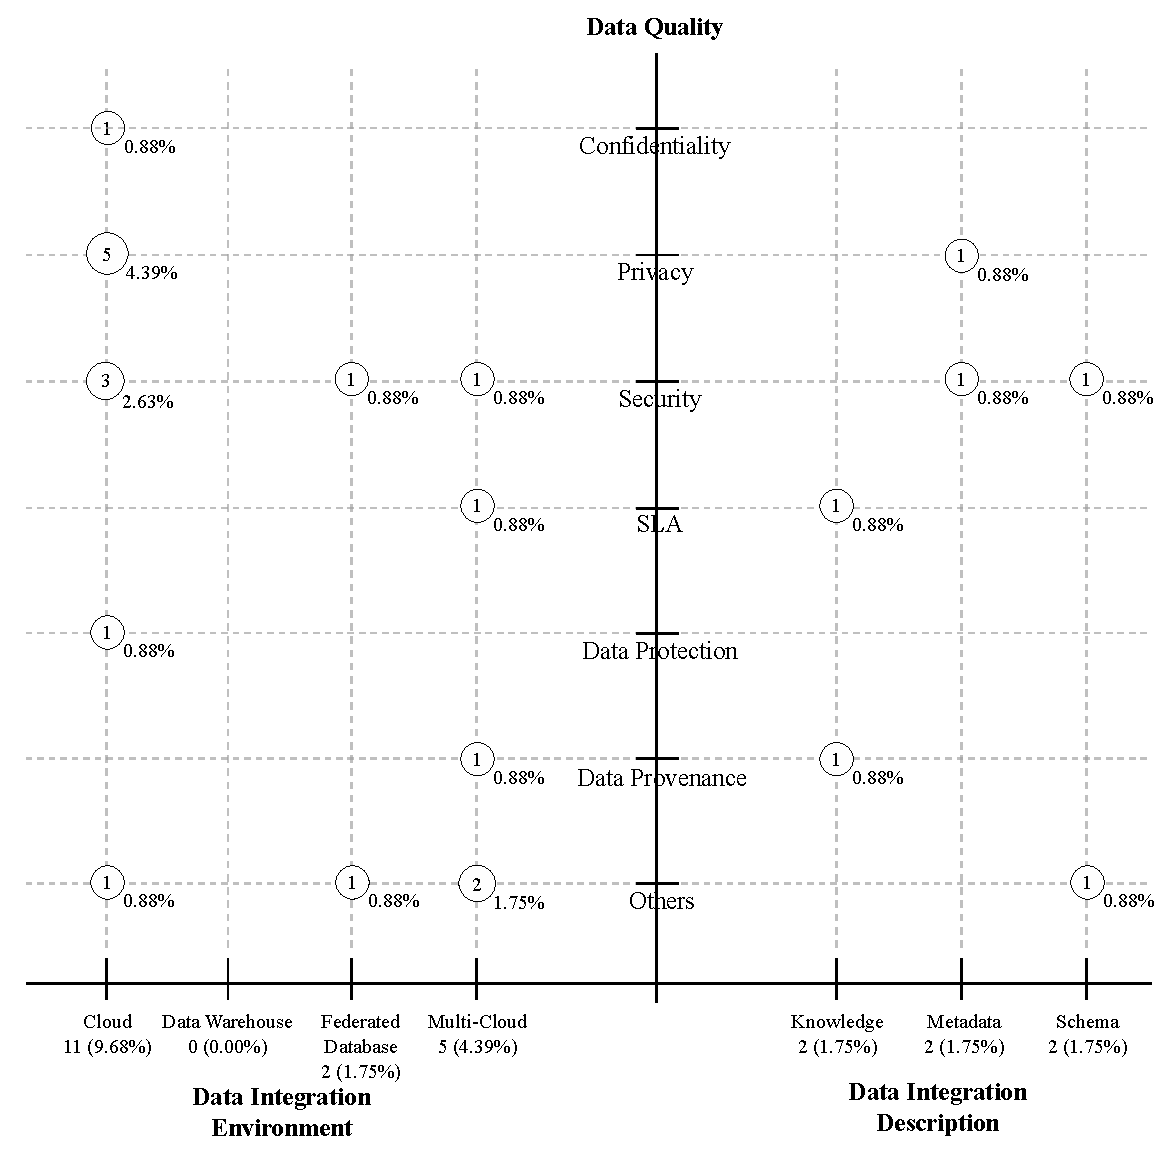
\includegraphics[scale=0.53]{figs/bubble-charts/Data-Quality-DI.pdf}
\caption{Facets Data Quality, Data Integration Environment and Data Integration Description}\label{fig:facet4}
\end{figure}

Combining the facet data quality with the facets data integration environment and data integration description
(Figure~\ref{fig:facet4}) it is possible to determine iIn which way and in which context has data integration been linked to QoS measures in the literature, particularly when associated to data integration environments like cloud  (9.68\%) and multi-cloud (4.39\%).

% \textit{Security} and \textit{privacy} the QoS measures that are most discussed together with data integration
 %(5 papers - 4.39\%). 
%The figure also shows that SLA has not been widely used in order to address data integration solutions
%(1 appearance) which reinforces our main objective of integrate SLA, data integration and multi-cloud 
%environments. 
%Analyzing the figure is also possible to observe that the most deployed data integration environment is 
%the cloud (9.68\%) followed by multi-cloud (4.39\%), federated databases (1.75\%) and data warehouse (0.00\%).
%The data integration description dimensions had the same percentage for schema, knowledge and metadata (2 appearance - 1.75\%)

% Most data integration environment consider cloud for solution. 
% 
% The type of contribution envolving data integration most often are
% \textit{tools} and \textit{models}, respectively. Some few others focus on the
% proposition of \textit{methods} or \textit{process}. 
